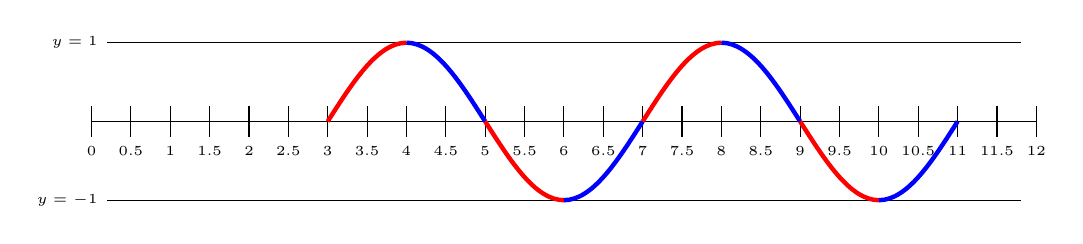
\begin{tikzpicture}

    \draw (0,0) -- (12,0);
    \draw (0.2,1)node[left,font=\tiny] {$y=1$} -- (11.8,1);
    \draw (0.2,-1)node[left,font=\tiny] {$y=-1$} -- (11.8,-1); 
    \foreach \x in {0,0.5,...,12}{
    \draw (\x,-0.2)node [below,font=\tiny,] {\x} -- (\x,0.2) ;
    }
    \draw[ultra thick, red] (3,0) sin (4,1);    %% the real business in this line
    \draw[ultra thick, blue] (4,1) cos (5,0);    %% the real business in this line
    \draw[ultra thick, red] (5,0) sin (6,-1);    %% the real business in this line
    \draw[ultra thick, blue] (6,-1) cos (7,0);    %% the real business in this line
    \draw[ultra thick, red] (7,0)  sin (8,1);    %% the real business in this line
    \draw[ultra thick, blue] (8,1) cos (9,0);    %% the real business in this line
    \draw[ultra thick, red] (9,0) sin (10,-1);    %% the real business in this line
    \draw[ultra thick, blue] (10,-1) cos (11,0);    %% the real business in this line
\end{tikzpicture}